\documentclass[12pt,a4paper]{article}
\usepackage[italian]{babel}
\usepackage[T1]{fontenc}
\usepackage[latin1]{inputenc}
\usepackage{graphicx}
\usepackage{amsmath}
\usepackage{subfig}
\usepackage[a4paper,top=1.5cm,bottom=1.4cm,left=1.4cm,right=1.4cm]{geometry}
\date{}
\begin{document}
\title{Ipersonica\\ Esercitazione 7 \\ Prof.re Renato Paciorri}
\author{Matteo Hakimi 1455230}
\maketitle
\begin{figure}[htbp]
\centering
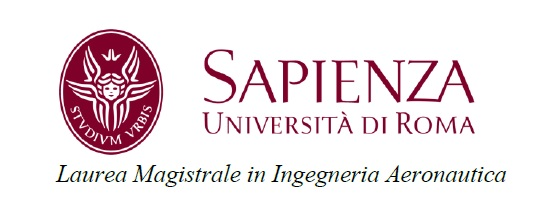
\includegraphics[width=100mm]{Immagini/1}
\end{figure}
\newpage
\tableofcontents
\newpage
\section{Introduzione}
Si vogliono ottimizzare le prestazioni aerodinamiche di un velivolo da crociera ipersonico, attraverso la riduzione della resistenza aerodinamica.
In particolare si cerca la forma ottima del velivolo tale che il coefficiente di resistenza a portanza nulla del velivolo risulti minimo.



\section{Formulazione del problema}
 Mentre nel problema del rientro la necessit� di frenare la capsula e di limitare lo scambio termico sono in accordo tra loro, in termini di geometria, nella crociera ipersonica il problema termico e aerodinamico entrano in conflitto. Si ricordi infatti come il flusso termico decada con l'inverso del raggio di curvatura.
 Supponiamo ora di considerare solo la parte aerodinamica.\\
 Uno dei parametri caratterizzanti le prestazioni del velivolo da crociera in termini di aerodinamica, � l'efficienza aerodinamica $E=\frac{L}{D}$. \\In particolare quello che si cerca di fare, nel caso di velivoli da crociera � quello di aumentare l'efficienza massima $E_{MAX}$.\\
 Partendo dalla polare del velivolo (si veda figura ), dalla definizione di efficienza aerodinamica risulta chiaro come l'efficienza massima sia legata al coefficiente angolare della retta tangente alla polare stessa.\\
 \begin{figure}[htbp!]
 	\centering
 	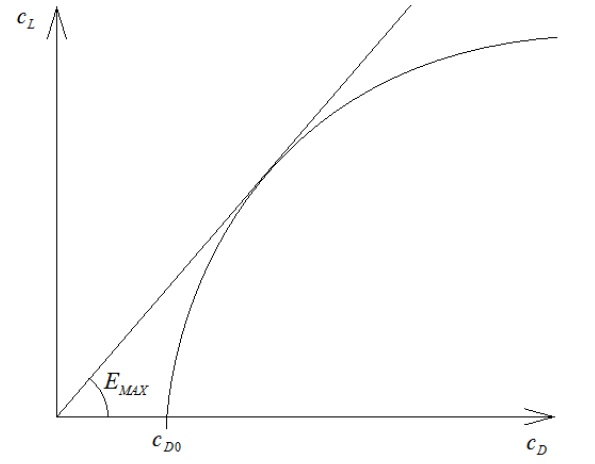
\includegraphics[width=100mm]{Immagini/polare}
 	\caption{Polare}
 \end{figure}\\
Nel contributo alla resistenza aerodinamica totale $D$, si considerano:\\
$\bullet$\quad resistenza di pressione $D_{p}$ \\
$\bullet$\quad resistenza viscosa $D_{v}$\\
Inoltre si ha:\\
$$D_{p}=D_{L}+D_{s}$$
dove $D_{L}$ � la resistenza dovuta alla generazione di portanza e $D_{s}$ � quella di forma.\\
Si ricava quindi:
$$D=D_{v}+D_{s}+D_{L}=D_{0}+D_{L}$$
avendo indicato con $D_{0}=D_{s}+D_{v}$ la resistenza a portanza nulla.\\
Adimensionalizzando si ha:\\
$$C_{D}=C_{D_{0}}+C_{D_{L}}$$
ovvero:\\
$$C_{D}=C_{D_{0}}+k\alpha^2$$
Osservando la polare di figura 1 si nota come per aumentare l'efficienza massima un modo pu� essere minimizzare la resistenza (coefficiente di resistenza) di portanza nulla.\\
\begin{figure}[htbp!]
	\centering
	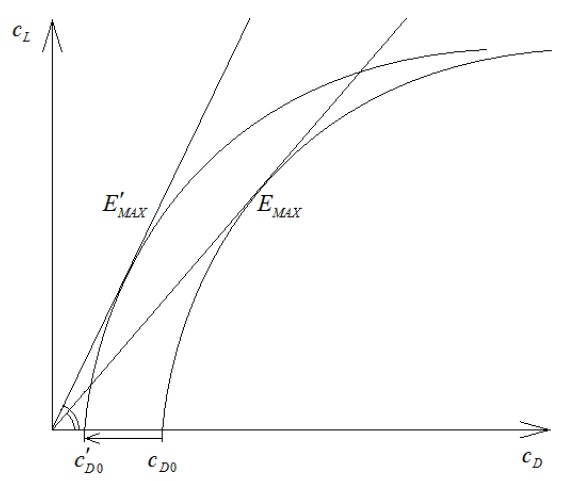
\includegraphics[width=100mm]{Immagini/polare1}
	\caption{Aumento dell'efficienza massima}
\end{figure}

Al fine di diminuire il $C_{D_{0}}$, si potrebbe intervenire sul solo termine viscoso, ad esempio facendo lavorare il corpo di
interesse in campo laminare a parit� di numero di Reynolds, agendo sulla finitura superficiale o minimizzando la superficie bagnata ed
abbassando cos� il coefficiente di attrito $c_{f}$. Oppure si potrebbe pensare di ridurre la resistenza di forma, facendo un corpo pi� allungato nella direzione di efflusso a parit� di volume.
Bisogna osservare come entrambi i metodi entrano in disaccordo, poich� diminuire il coefficiente di attrito cercando di far lavorare il corpo in campo laminare potrebbe essere sconveniente in termini di resistenza di forma; infatti il passaggio a regime turbolento, favorisce il ritardo della separazione del flusso sul corpo, riducendo la scia a valle dello stesso. Allo stesso modo cercare di diminuire il coefficiente di attrito dimunendo la superficie bagnata, avendo fissato il volume del corpo, da origini a corpi di natura tozza e quindi soggetti a maggior resistenza di forma. Viceversa, favorendo l'allungamento del velivolo, a parit� di volume, al fine di diminuire la resistenza di forma, ha il duplice effetto di aumentare la resistenza di attrito a causa dell'aumento della superficie bagnata.\\
Da quanto detto sopra si evince che bisogna trovare un compromesso per cercare di non estremizzare i due effetti e minimizzare globalmente il coefficiente di resistenza a portanza nulla.
Si parte dal concetto di lastra piana, che rappresenta la forma pi� aerodinamica possibile, e ci si allontana da questa al fine di realizzare un corpo con un certo
volume interno.\\
\newpage
Si parte con un semplice diedro visto in sezione. 
\begin{figure}[htbp!]
	\centering
	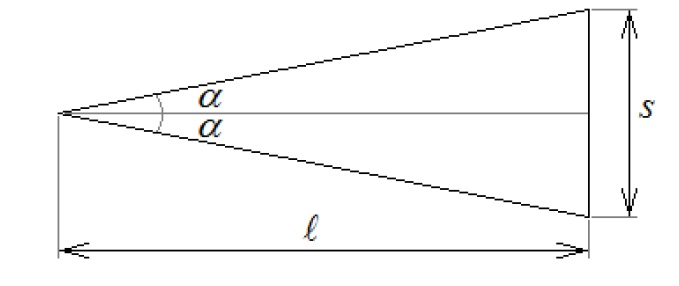
\includegraphics[width=100mm]{Immagini/diedro}
	\caption{Corpo diedro visto in sezione}
\end{figure}\\
Cerchiamo ora di stimare gli andamenti del coefficiente di resistenza di forma e viscoso al variare del rapporto delle lunghezze caratteristiche del corpo $s$ e $l$.\\
 Fissando come vincolo di volume $s\cdot l=0.1 m^2$ (caso 2D), si ha:\\
 $\bullet$\quad {\bf Resistenza di forma}
 Il flusso tipico che si viene a creare in prossimit� del corpo per $M>1$ � il seguente:\\
 \begin{figure}[htbp!]
 	\centering
 	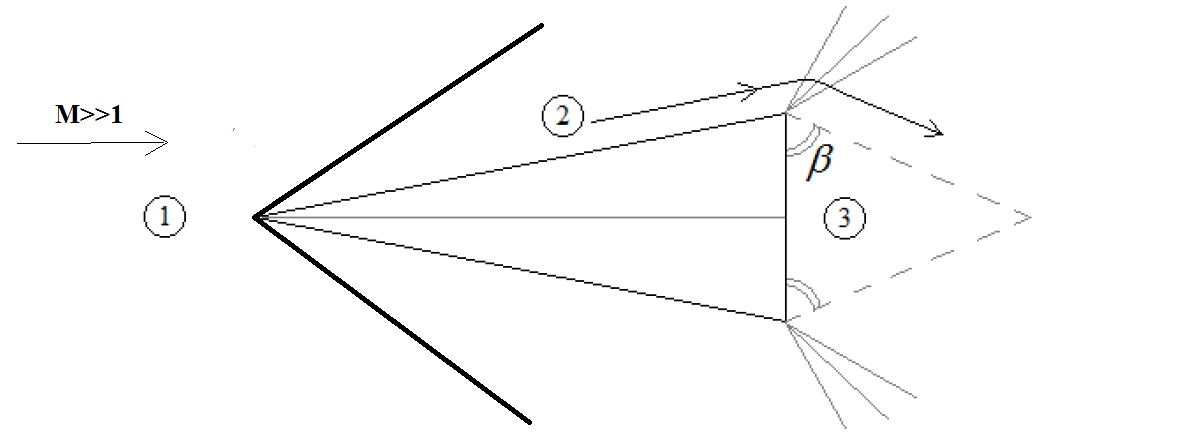
\includegraphics[width=100mm]{Immagini/flusso}
 	\caption{Flusso 2D attorno a diedro}
 \end{figure}\\
 In particolare si ha:\\
 $$D_{s}=(p_{2}-p_{3})\cdot s\approx p_{2}\cdot s$$
Dove la pressione $p_{3}$ � stata trascurata rispetto a $p_{2}$ poich� l'espansione a valle del corpo sar� molto violenta. In particolare se avessimo stimato la resistenza di forma con la teoria Newtoniana avremo trovato che $p_{3}=p_{1}<<p_{2}$ per $M_{1}>>1$.\\
Dall'espressione del coefficiente di resistenza di forma si ricava:\\
$$C_{D_{s}}=\frac{D_{s}}{\frac{1}{2}\rho_{1}U_{\infty}^2s}=\frac{\frac{p_{2}}{p_{1}}}{\frac{1}{2}\gamma M_{1}^2}$$
Attraverso il parametro di similitudine ipersonica $k=\alpha M$, con $\alpha\approx\frac{s}{2l}=\frac{1}{2\frac{l}{s}}$ tangente locale, si ha:\\
$$\frac{p_{2}}{p_{1}}=1+\gamma k^2\left[\frac{\gamma+1}{4}+\sqrt{\left(\frac{\gamma+1}{4}\right)^2+\frac{1}{k^2}} \right]$$
ovvero:\\
$$C_{D_{s}}=f(\frac{l}{s})$$
$\bullet$\quad {\bf Resistenza viscosa}
Supponendo $\alpha$ sufficientemente piccolo, possiamo trattare il corpo come una doppia lastra piana.\\
Possiamo quindi scrivere:\\
$$D_{v}=2\cdot\left[\frac{1}{2}\rho_{1}U_{\infty}^2c_{f}l\right]$$
Dove $c_{f}$ � il coefficiente di attrito, dipendente dal regime dal numero di Reynolds e dal regime di moto.\\
Nell'ipotesi che il flusso sia laminare possiamo scrivere:\\
$$c_{f}=\frac{1.24}{\sqrt{Re_{l}}}$$
avendo indicato con $Re_{l}=\frac{\rho_{1}U_{\infty}l}{\mu_{1}}$.
Da cui si ricava:\\
$$C_{D_{v}}=\frac{D_{v}}{\frac{1}{2}\rho_{1}U_{\infty}^2s}$$
Si noti come l'adimesionalizzazione � stata fatta rispetto a $s$ e non a $l$, questo perch� cosi � possibile confrontare il $C_{D_{s}}$ con il $C_{D_{v}}$.
Sapendo che $l=\sqrt{0.1\frac{l}{s}}$, si ricava:\\
$$C_{D_{v}}=2\frac{1.24}{\sqrt{\frac{\rho_{1}U_{\infty}}{\mu_{1}}}\sqrt[4]{0.1}}\left(\frac{l}{s}\right)^{3/4}$$
$\bullet$\quad {\bf Resistenza a portanza nulla}
Come visto nella sezione precedente, la resistenza in assenza di portanza � la somma dei contributi di resistenza di forma e viscosa rispettivamente.\\ In particolare, in termini di $C_{D}$ si ha:\\
$$C_{D_{0}}=C_{D_{v}}+C_{D_{s}}=f(\frac{l}{s})$$
In particolare si riporta l'andamento del coefficiente di resistenza al variare di $\frac{l}{s}$.
 \begin{figure}[htbp!]
 	\centering
 	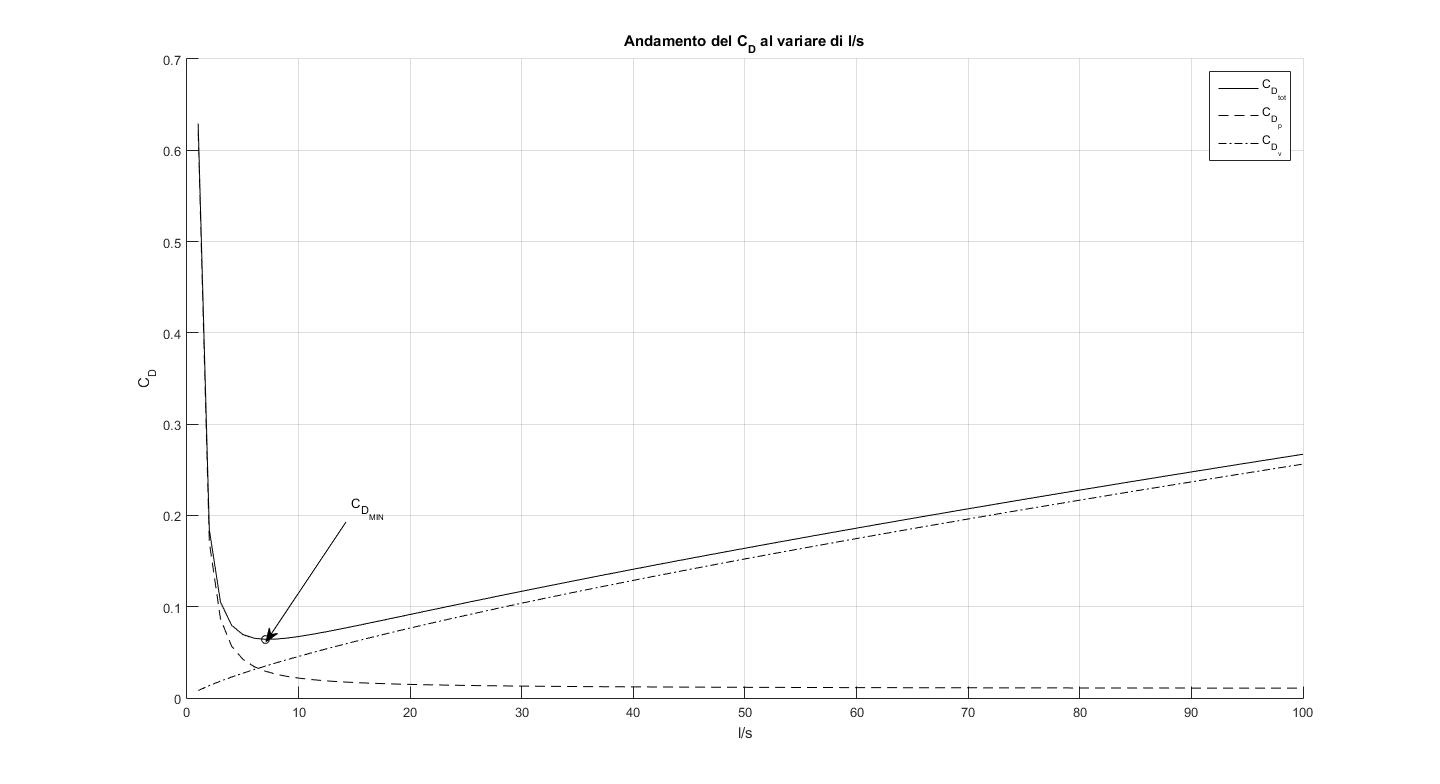
\includegraphics[width=150mm]{Immagini/CD}
 	\caption{Andamento del $C_{D_{0}}$ al variare del rapporto $l/s$ }
 \end{figure}\\
Si nota come in tale andamento si abbia la presenza di un minimo. Chiaramento quello � il punto di ottimo.\\
\section{Ottimizzazione della forma}
Nella sezione precedente si � fatto uno studio su come minimizzare il coefficiente di resistenza, in assenza di portanza, al fine di aumentare l'efficienza massima del velivolo ipersonico da crociera. Tuttavia nello studio precedente sono state assunte diverse ipotesi; prima tra tutte, si � detto che la forma di minima resistenza aerodinamica � quella data del diedro, questo � vero in condizioni di problemi bidimensionali. In realt� si dimostrer� che la forma ottima nel caso 3D � data dalla geometria assialsimmetrica dell'Ogiva.\\
In generale, si pu� prendere un profilo con legge $y=y(x)$ con un vincolo sul volume, oppure un vincolo che fissi i punti iniziale e finale del profilo. Si otterr� una famiglia di curve che potr� essere riscalata in base al volume necessario.\\

 \begin{figure}[htbp!]
 	\centering
 	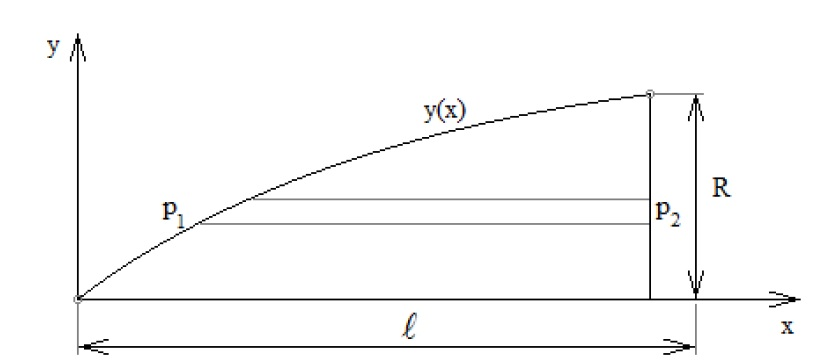
\includegraphics[width=100mm]{Immagini/profilo}
 	\caption{Profilo generico $y=y(x)$}
 \end{figure}

Per calcolare la resistenza per unit� di profondit� si prende il contributo elementare di una
porzione orizzontale del profilo, come in figura.\\
Si ricava che nel caso $2D$.
$$D=\int_{0}^{R}\left(p_{1}-p_{2}\right)dy$$
ovvero:\\
$$C_{D}=\frac{D}{\frac{1}{2}\rho_{1}U_{\infty}^2R}=\frac{1}{R}\int_{0}^{R} \frac{2}{M_{\infty}^2\gamma}\left(\frac{p_{1}}{p_{\infty}}-\frac{p_{2}}{p_{\infty}}\right)dy$$
Se $M_{\infty}>>1$ allora potendo utilizzare la teoria Newtoniana si ha $p_{2}=p_{\infty}$ da cui si ricava:\\
$$C_{D}=\frac{1}{R}\int_{0}^{R} \frac{2}{M_{\infty}^2\gamma}\left(\frac{p_{1}}{p_{\infty}}-1\right) dy$$ 
Si riconosce come il termine integrando sia il coefficiente di pressione $C_{p}$.
Sempre dalla teoria Newtoniana si ha:\\
$$C_{p}=2sin^2(\delta)$$
Sappiamo inoltre che:\\
$$y'=\frac{dy}{dx}=tg(\delta)$$
ovvero:\\
$$sin^2(\delta)=\frac{y'^2}{1+y'^2}$$
Da cui si ha che:\\
$$C_{D}=\frac{2}{R}\int_{0}^{L}\frac{y'^3}{1+y'^2}dx$$
avendo posto $dy=y'dx$\\
Nel caso assialsimmetrico si ha invece
$$C_{D}=4\int_{0}^{L}\frac{y'^3y}{1+y'^2}dx$$
Per risolvere il problema della ricerca del minimo si imposta un problema variazionale attraverso
la definizione del funzionale $V$.
$$V=V[y(x)]=\int_{x_{1}}^{x_{2}}F(x,y,y')dx$$
Nel caso generale usando i moltiplicatori di Lagrange si ha:\\
$$\frac{\partial F}{\partial y}-\frac{\partial^2 F}{\partial y \partial x}-\frac{\partial^2 F}{\partial y \partial y'}y'-\frac{\partial^2 F}{\partial^2 y}y''=0$$
Per quanto riguarda il caso piano si ha:
$$F=\frac{y'^3}{1+y'^2}=F(y')$$\\
e il problema si riduce a:\\
$$\frac{\partial^2 F}{\partial^2 y}y''=0$$
ovvero:\\
$$y''=0$$
da cui si ha:\\
$$y=Ax+B$$
con $A$ e $B$ dipendenti dalle condizioni al contorno che nel nostro caso sono:\\
$$y(0)=0,\quad y(L)=R$$
Si osserva come nel caso piano abbiamo ottenuto una legge lineare, questo corrisponde al fatto che per minimizzare la resistenza nel caso piano bisogna adottare la forma del diedro.\\
Per quanto riguarda il caso assialsimmetrico le cose cambiano.\\ In particolare si ha:\\
$$F=F(y,y')$$
che sositutita nella formula ottenuta dal problema di minimo variazionale si pu� dimostrare che:\\
$$\frac{yy'^3}{(1+y'^2)^2}=cost$$
Provando una soluzione del tipo $y=kx^{3/4}$ si ha:\\
$$\frac{\frac{3}{4}}{\left[1+\frac{3}{4}^2\frac{1}{\sqrt{x}}\right]^2}$$
Osserviamo come tale soluzione non soddisfi la relazione ottenuta precedentemente.\\
Tuttavia sufficientemente lontano dall'origine approssima molto bene la soluzione.\\
Un altro modo di procedere � derivare la relazione ottenuta rispetto a x. In particolare si ha:\\ 
$$y''=\frac{y'^2(1+y'^2)}{y(y'^2-3)}$$
Ponendo $A=y'$ si ottiene il seguente sistema del primo ordine:\\
$$y'=A\\A'=\frac{A^2(1+A^2)}{y(A^2-3)}$$
con le seguenti condizioni al contorno:\\
$$y(0)=0,\quad y(L)=R$$
Al fine di implementare il sistema differenziale, in ambiente Matlab, il problema ai limiti viene ricondotto ad un problema ai valori iniziali iterando sul valore di $A(0)=A_{it}$.
In realt� bisogna osservare come nel sistema di equazioni sia presente una singolarit� in $y(0)=0$, per cui ponendo $y(0)=0.0001$ e scegliendo $L=1$ e $R=0.1$ si ha che $A_{it}=0.3795$.\\
Vengono riportati i risultati in forma grafica confrontati con l'approssimazione $y=x^{3/4}$.\\
 \begin{figure}[htbp!]
 	\centering
 	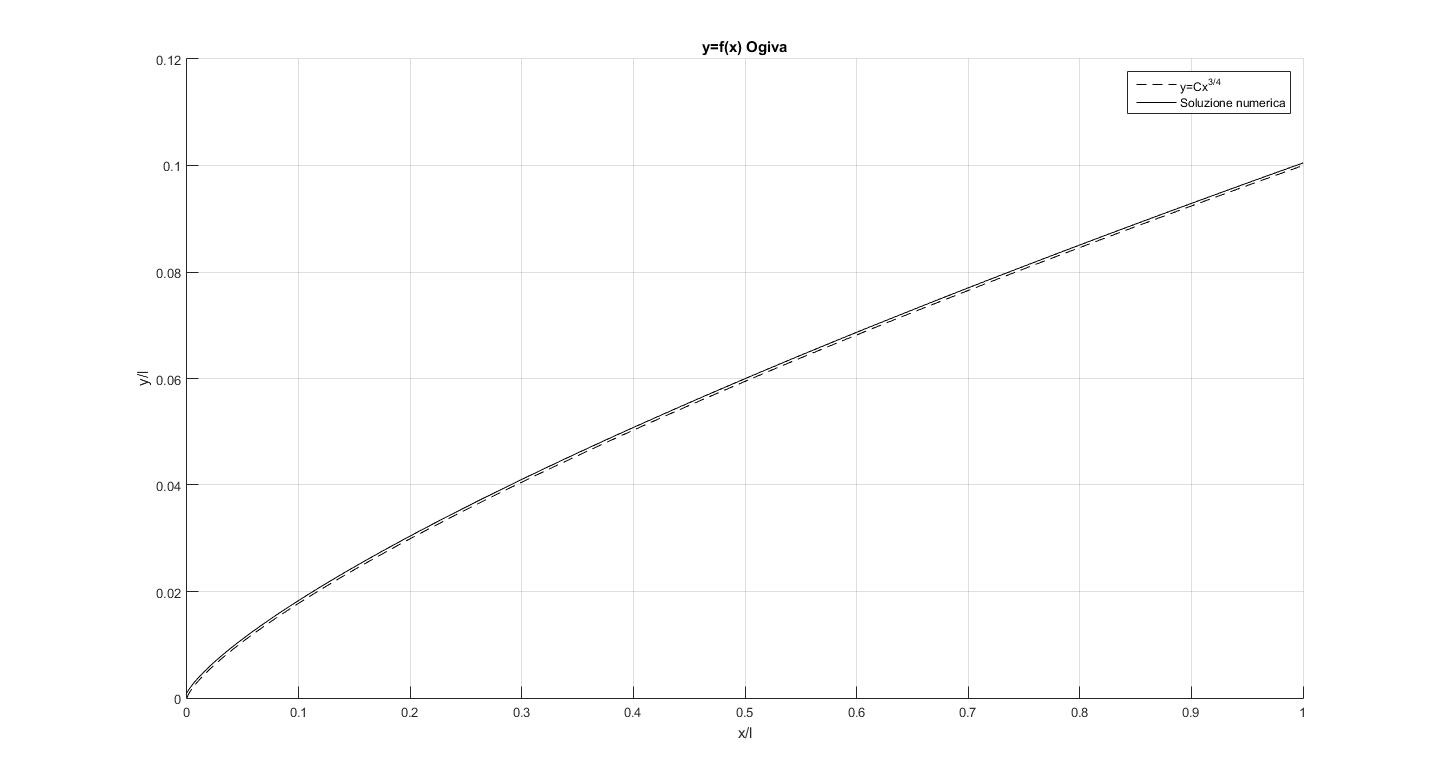
\includegraphics[width=150mm]{Immagini/ogiva}
 	\caption{Profilo ogiva soluzione numerica e $y=cx^{3/4}$}
 \end{figure}\\ 
Il motivo fisico per cui l'ogiva risulta pi� vantaggiosa rispetto ad un semplice cono sta nel fatto che nell'ogiva la pressione diminuisce lungo la direzione del flusso. Infatti, dato che la pressione a valle dipende dall'inclinazione della superficie, per il cono la pressione si mantiene costante lungo le sue generatrici, mentre per l'ogiva la pendenza scende gradualmente.
Inoltre si pu� affermare che, nonostante il cono occupi meno volume a parit� di larghezza, esso presenta maggiore resistenza. Infatti sul cono un contributo $dp$ alle alte x contribuisce molto
alla resistenza totale, sia perch� la corona circolare ivi � grande, sia perch� il dp insiste su una dy grande. L'ogiva, invece, ha pendenze alte dove la corona � piccola e d� pi� bassi contributi a valle a parit� di ascissa con il cono.
 
 
 
\end{document}